\section{Experimental Setup}

\begin{figure*}
    \centering
    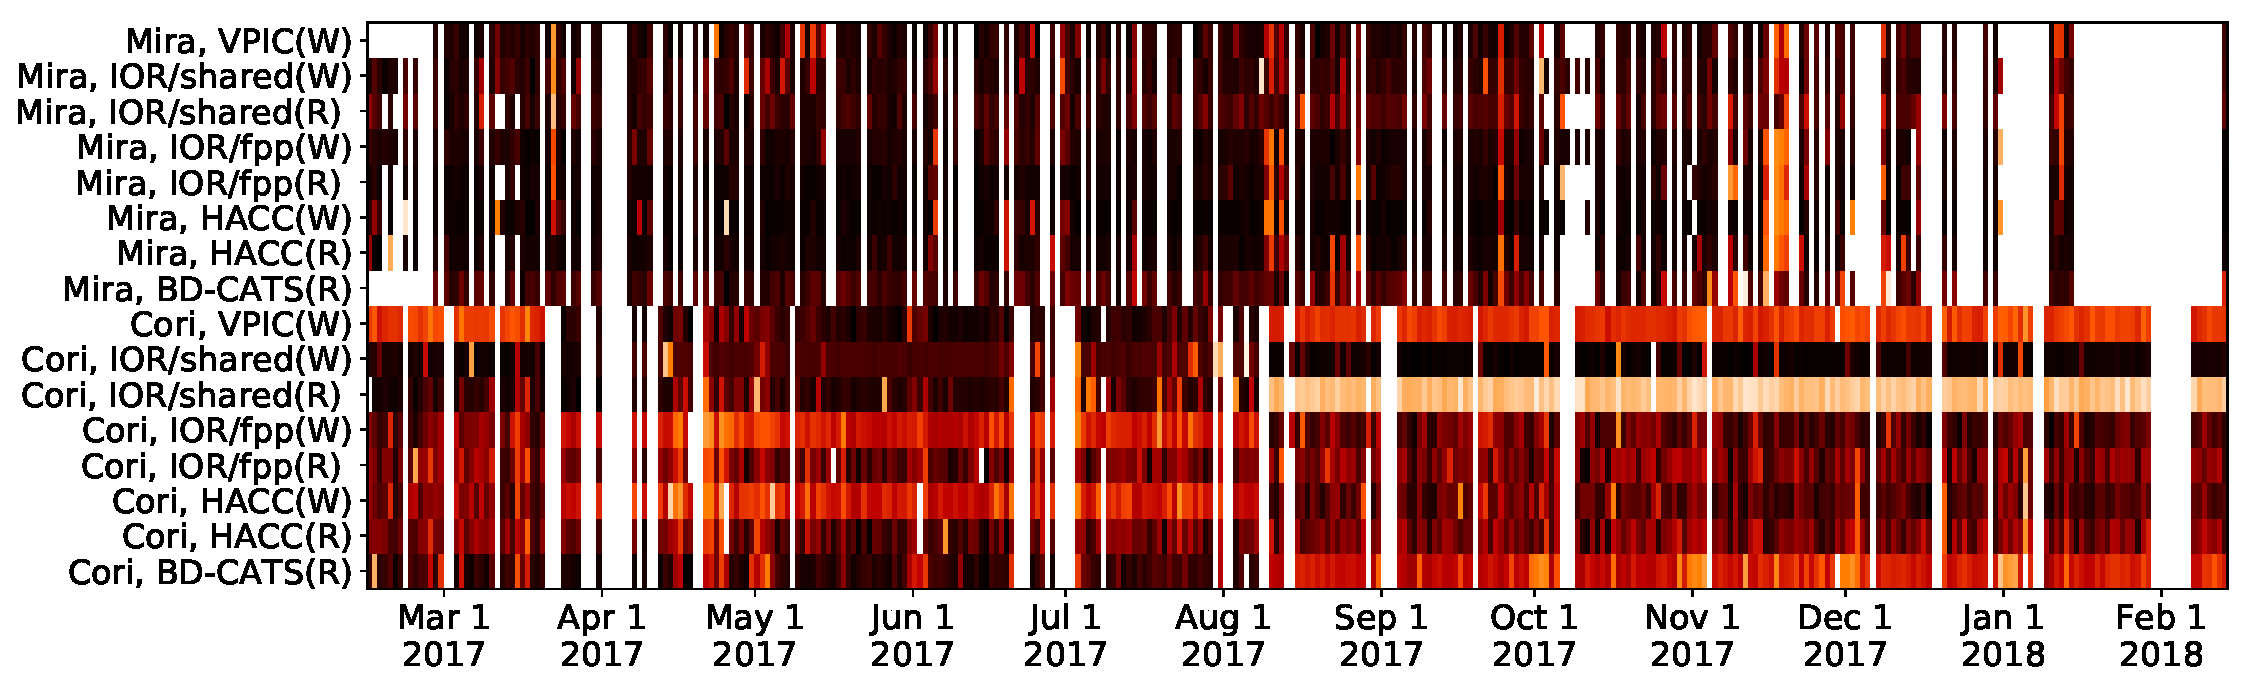
\includegraphics[width=0.90\linewidth]{summary_heatmap}
    \vspace{-.2in}
    \caption{Performance of daily benchmarks normalized to each benchmark's peak observed performance on the specified storage system.  Lighter colors represent lower performance, and whitespace represents benchmarks that did not run.  Performance is normalized only within each row.}
    \TODO{colored sparklines might be more effective here}
    \label{fig:summary-heatmap}
%   \vspace{-.3in}
\end{figure*}

\TODO{How about changing this to ``Methodology'' section and have 'Data collection', 'Data characteristics', and 'Data analysis methods' as subsections, to make it sound this is the novel contribution of this effort? -- Suren}

\TODO{Rely on PDSW paper and upcoming CUG submission on TOKIO to provide lower level details, summarize high-level concepts most relevant to this study.}

\TODO{Does this paragraph need to be moved into related work or otherwise reworded?}
Previously, we have demonstrated the feasibility of a general approach to holistic I/O analysis of HPC systems and applied that approach over a month-long benchmarking study to examine specific cases of anomalous I/O behavior and to deduce potential factors contributing to this behavior~\cite{Lockwood2017}. We later formalized our methodology with the specification of the TOKIO (Total Knowledge of I/O) framework~\cite{Lockwood2018tokio}. For this study, we build on our prior research and use TOKIO to analyze a massive amount of I/O monitoring data culminating from a year-long benchmarking study conducted on a number of leadership-class HPC systems. 

In the following sections, we provide an overview of TOKIO, describe the production HPC platforms we have deployed it on at NERSC and the ALCF, and describe the benchmarking methodology  utilized in this study.

\subsection{TOKIO Overview}

%A holistic approach to understanding I/O behavior is a necessity given the move towards more complicated I/O architectures (in terms of number of constituent components, like high-level I/O libraries, I/O middleware systems, and low-level storage hardware) on these systems. TOKIO's primary goal is to arm system users, administrators, and I/O researchers with the necessary tools to navigate this complexity and to make meaningful observations into how workloads interact with the I/O subsystem.

TOKIO is a framework facilitating holistic characterization and analysis of I/O workloads running on today's production HPC systems. Conceptually, it provides an abstraction layer between component-level monitoring tools already deployed on HPC platforms and higher-level I/O analysis tools that utilize this data. The fundamental roles of the TOKIO framework are to: collate monitoring data from distinct comonents; integrate and normalize the data from these components (each with its own native format, scope, and granularity); and present coherent interfaces for indexing and accessing this data.

TOKIO also has its own data format specification for I/O monitoring data and has tools for archiving timeseries data in this format.

TOKIO's modular architecture simplifies the process of integrating new monitoring sources into the framework, providing users access to a rich set of data characterizing holistic I/O behavior on systems in which it is deployed. Currently, TOKIO offers interfaces with the following monitor sources \footnote{We refer readers to our previous work~\cite{Lockwood2017, Lockwood2018tokio} for a more detailed description of the monitoring sources TOKIO supports.}:

\begin{itemize}
\item application-level monitoring
  \begin{itemize}
  \item Darshan~\cite{Carns2009} provides a condensed set of I/O counters and statistics for each file accessed by a given application. 
  \end{itemize}
\item file system workload monitoring
  \begin{itemize}
  \item LMT
  \item ggiostats
  \end{itemize}
\item file system health and capacity monitoring
\item job scheduler data
\item \TODO{burst buffer monitoring?}
\end{itemize}

\TODO{Worth giving the shoutout to the pytokio implementation here, or does that go in the reproducibility appendix?}

\subsection{HPC Platforms}

\TODO{Describe Mira and Edison, and the file systems being studied.}

\subsection{I/O Benchmarks}

We ran the benchmarks described in~\cite{Lockwood2017} daily from February 14, 2017 to February 15, 2018 (366 days) and generated 11,986 Darshan logs across Mira, Cori, and Edison.  This reflects 81.9\% of the intended benchmark runs having generated results.
The 18.1\% of missing benchmarks resulted from system downtime, malfunctions of component-level monitoring tools or the automated test scheduling, queue wait times that exceeded 24 hours, and benchmarks exceeding their walltime.
The fact that no results were obtained for jobs that ran so slowly that they exceeded their reserved walltime is significant in that this dataset does not capture the absolute worst performance observed.
Although not ideal, this reflects the realities of daily testing on production systems.

An overview of the performance measurements is shown in Figure \ref{fig:summary-heatmap}.

\TODO{Things that are important here: behavior over time, grouping data
sources in a way that helps understand scope, focusing on fundamental
\emph{changes} in performance rather than steady state, everything in one
view.}

%\begin{figure}[t]
%    \centering
%    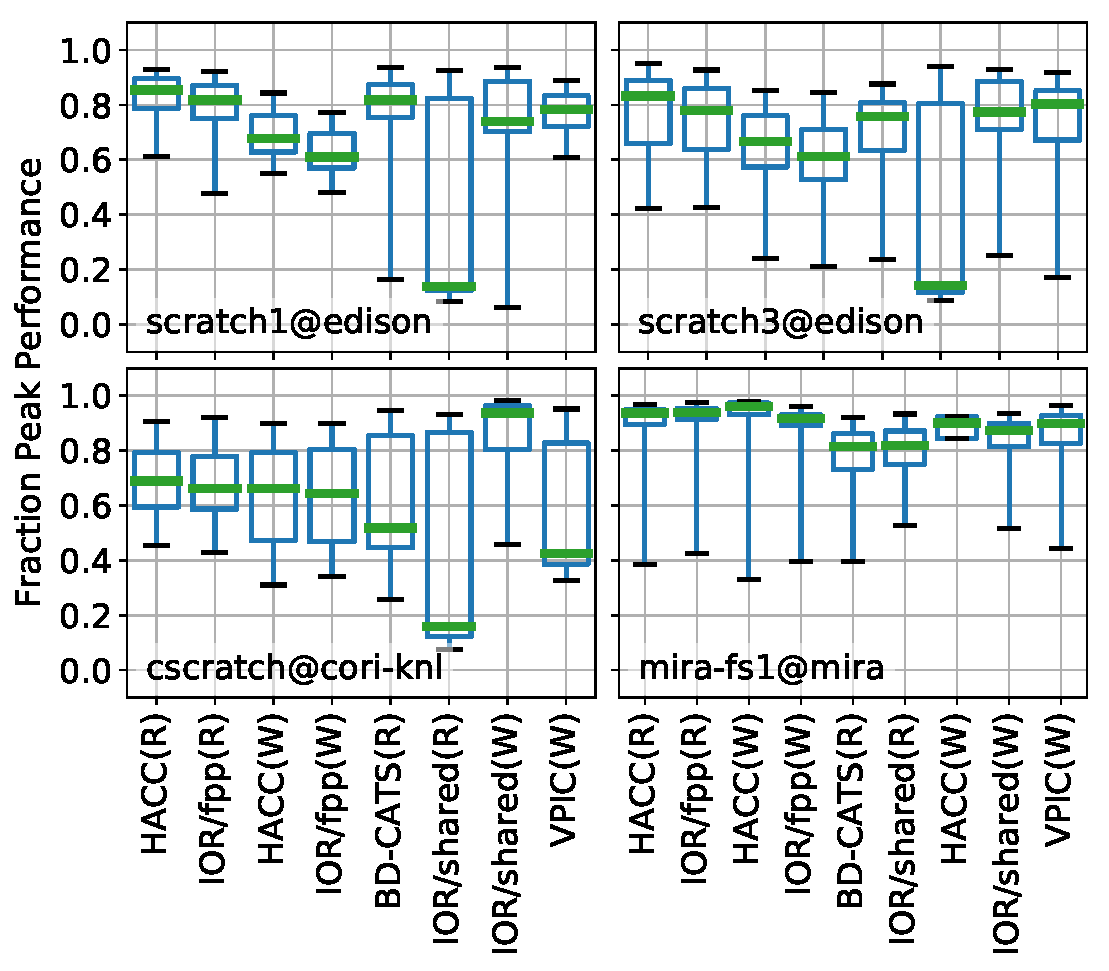
\includegraphics[width=1.0\columnwidth]{summary_boxplots}
%    \vspace{-.35in}
%    \caption{I/O performance grouped by test applications and read(R)/write(W) mode.  Whiskers represent the 5th and 95th percentiles.}
%    \label{fig:summary-boxplots}
%%   \vspace{-.3in}
%\end{figure}\
